\documentclass[10pt,table,dvipsnames]{beamer}
\usepackage{tikz}
\usepackage{mathptmx}
\usepackage[scaled=0.94]{helvet}
\usepackage[absolute,overlay]{textpos}
\usepackage{hyperref}
\usepackage{listings}
\lstloadlanguages{python}

\author{S.~Poss}
\title{ILCDIRAC}
\subtitle{A grid solution for the LC community}
\date{Jan 29, 2013}
\institute{CERN, LAPP}
\newcommand{\interstitial}[1]{\begin{frame}\begin{block}{}\centering\Huge{#1}\end{block} \end{frame}}
\newcommand{\backupslides}{\interstitial{Backup Slides}}

\mode<all>
\TPGrid{50}{50}

\pgfdeclareimage[width=0.1\paperwidth]{cliclogo}{CLIClogo}
\newcommand{\ClicLogo}{%
\begin{textblock}{14}(45., 0.05)
 \href{http://lcd.web.cern.ch}{\pgfuseimage{cliclogo}}
\end{textblock}
}

\setbeamertemplate{footline}
{%
  \leavevmode%
  \hbox{%
  \begin{beamercolorbox}[wd=.222222\paperwidth,ht=2.25ex,dp=1ex,left]{title in 
head/foot}%
    \usebeamerfont{date in head/foot}\insertshortdate{}\hspace*{2em}
  \end{beamercolorbox}%
  \begin{beamercolorbox}[wd=.555555\paperwidth,ht=2.25ex,dp=1ex,center]{author 
in head/foot}%
    \usebeamerfont{author in head/foot}\insertshortauthor{}:
    \usebeamerfont{title in head/foot}\insertshorttitle
  \end{beamercolorbox}%
  \begin{beamercolorbox}[wd=.222222\paperwidth,ht=2.25ex,dp=1ex,right]{date in 
head/foot}%
    \insertframenumber{}/\inserttotalframenumber\hspace*{2ex}
  \end{beamercolorbox}}%
  %\vskip0pt%
  \ClicLogo
}

\beamertemplatenavigationsymbolsempty
\setbeamertemplate{blocks}[rectangle]
\setbeamersize{text margin left=1em,text margin right=1em}

%\setbeamertemplate{headline}[default]

\begin{document}
\renewcommand{\inserttotalframenumber}{\ref{lastframe}}

\begin{frame}
\titlepage
\end{frame}

\begin{frame}
\frametitle{Outline}
\tableofcontents
\end{frame}

\section{Introduction}\label{sec:intro}
\begin{frame}
  \frametitle{What is ILCDIRAC ?}
It's a \alert{DIRAC client} specific to the Linear Collider community:
\begin{itemize}
\item DIRAC is a {\color{NavyBlue}grid solution} initially developed for LHCb
\item Extended for {\color{NavyBlue}other communitites}: Belle 2, BES, ILC, FERMI-LAT,\\
  several biomed applications, etc.
\item \alert{Complete solution}: Job Management, File catalog, etc.
\end{itemize}
~\\
ILCDIRAC:
\begin{itemize}
\item Enables use of {\color{NavyBlue}ALL ILC software} on the grid in a {\color{NavyBlue}unified manner}
\item Use of {\color{NavyBlue}any available resource} (WLCG, OSG, local batch farms,
  etc.)
\item Comes with a {\color{NavyBlue}web portal} that allows for most operations
\end{itemize}
\end{frame}

\section{Job Management}
\label{sec:jobman}

\subsection{Using the python API}
\label{sec:api}

\begin{frame}
  \frametitle{Job Management with the python API}
Idea: \alert{Users need to care what to run, not how.}
\begin{itemize}
\item All ILC {\color{NavyBlue}applications are configured uniformly} thanks to a common interface
  \begin{itemize}
  \item {\color{ForestGreen} ``Applications'' share logical properties} like SteeringFile,
    Version, etc.\\
~\\
  \item {\color{ForestGreen}Application specific things} (Model, DST file name, etc.) have
    {\color{ForestGreen} dedicated setters}: they are only available to applications for
    which they make sense
  \end{itemize}
~\\
\item {\color{NavyBlue}Data can be accessed} from the catalog using {\color{NavyBlue}meta data queries}
  directly during job submission
  \begin{itemize}
  \item DIRAC File catalog has meta data information (and replica
    info), see later\\
  \end{itemize}
~\\
\item {\color{NavyBlue}Steering files} used for Production are {\color{NavyBlue}available directly} to the
  users
  \begin{itemize}
  \item Only the file names are needed
  \end{itemize}
~\\
\item {\color{NavyBlue}Output files} are stored in a user configurable directory,
  without need of Storage Element specification
  ({\color{NavyBlue}cloud-like})\\
~\\
\item Failover mechanism: \alert{produced files cannot be lost}:
  copied to another storage, and replication request is issued for
  later treatment
\end{itemize}
\end{frame}

\begin{frame}
  \frametitle{Simple job example: Marlin} 
\lstset{emph={Marlin,m,Applications,setVersion,setSteeringFile,setGearFile,setInputFile},emphstyle=\color{blue},
emph={[2]UserJob,j,append,submit},emphstyle={[2]\color{red}},
emph={[3]DiracILC,d},emphstyle={[3]\color{BurntOrange}}}
\lstinputlisting[language=python,basicstyle=\footnotesize]{SimpleJob.py} 
Complete examples and documentation in {\color{blue}http://www.cern.ch/lcd-data/doc/HeadFirstTalk.pdf}
\end{frame}

\subsection{Using the web portal}
\label{sec:web}

\begin{frame}
  \frametitle{Job Management with the Web portal}
  \begin{itemize}
  \item Possibility to {\color{NavyBlue}submit small jobs through the portal} directly
\end{itemize}
\centering
\includegraphics[width=0.7\textwidth]{JobMan2}~\\
\begin{itemize}
\item Interface to {\color{NavyBlue}monitor the statuses, apply some operations}
\item {\color{NavyBlue}Small sandboxes} can be obtained {\color{NavyBlue}from the portal}, big ones are
  stored on the GRID
\end{itemize}
\end{frame}

\subsection{Performance}
\label{sec:perfs}

\begin{frame}
  \frametitle{Performance: User jobs}
\centering
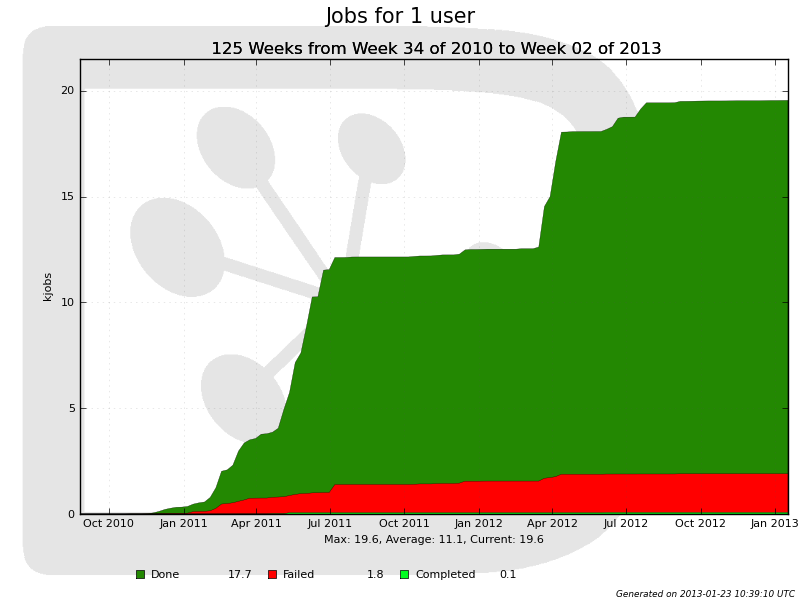
\includegraphics[width=.9\textwidth]{JobsJJ}\\
\end{frame}
\begin{frame}
  \frametitle{Performance: Production jobs}
\centering
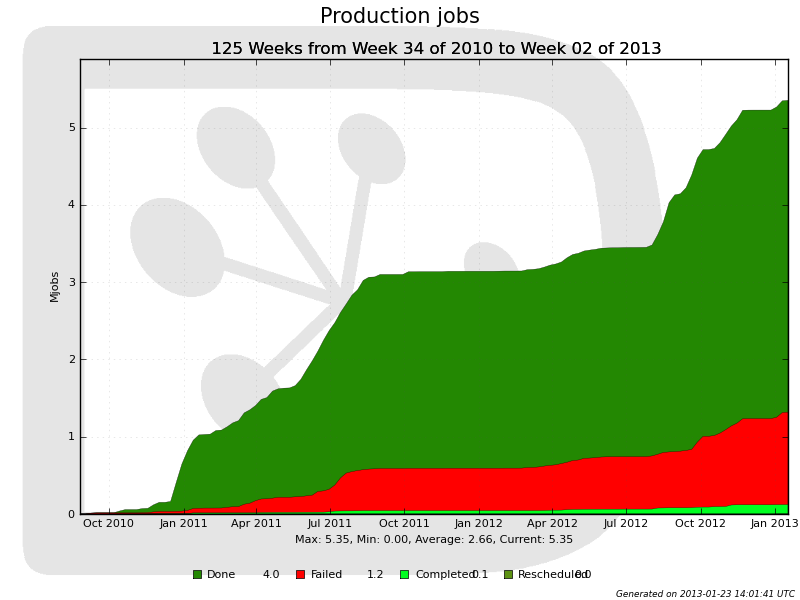
\includegraphics[width=0.9\textwidth]{JobsProd}\\
\end{frame}

\begin{frame}
  \frametitle{Performance: Total jobs}
\centering
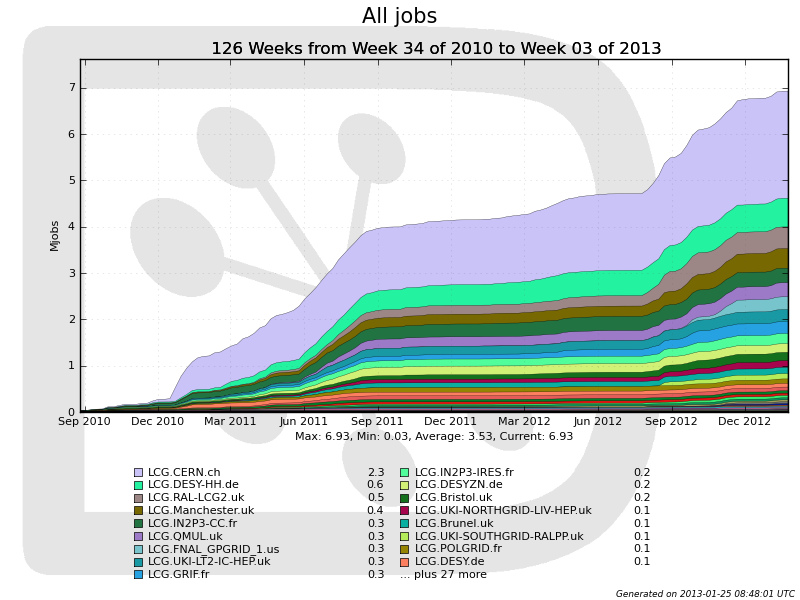
\includegraphics[width=0.9\textwidth]{JobsAll}\\
\end{frame}


\section{DIRAC File Catalog}
\label{sec:fc}

\subsection{Details}
\label{sec:fcdetails}

\begin{frame}
  \frametitle{DIRAC File catalog}
\begin{itemize}
\item Meta data catalog: {\color{NavyBlue}Directory and file level meta tags}
  \begin{itemize}
  \item Searchable (like Event type) and non searchable tags (like number of events)
  \item {\color{ForestGreen}Ancestor/daughter relationships}
  \end{itemize}
~\\
\item {\color{NavyBlue}Replica catalog}: Where the files are physically, with a path
  depending only on Storage Element logical name
  \begin{itemize}
  \item SE logical name is defined in the Configuration Service: {\color{ForestGreen}if an
    end-point changes its name, the files are not lost}
  \end{itemize}
\end{itemize}
~\\
File {\color{NavyBlue}Register operations} in ILCDIRAC now done {\color{NavyBlue}in the DFC and the Lcg File Catalog}
simultaneously (failover applies here too). \\
~\\
{\color{NavyBlue}ILC DBD files} in the LFC are synchronised in the DFC.
\end{frame}

\subsection{Web interface}
\label{sec:webfc}

\begin{frame}
  \frametitle{File catalog web interface}
\centering
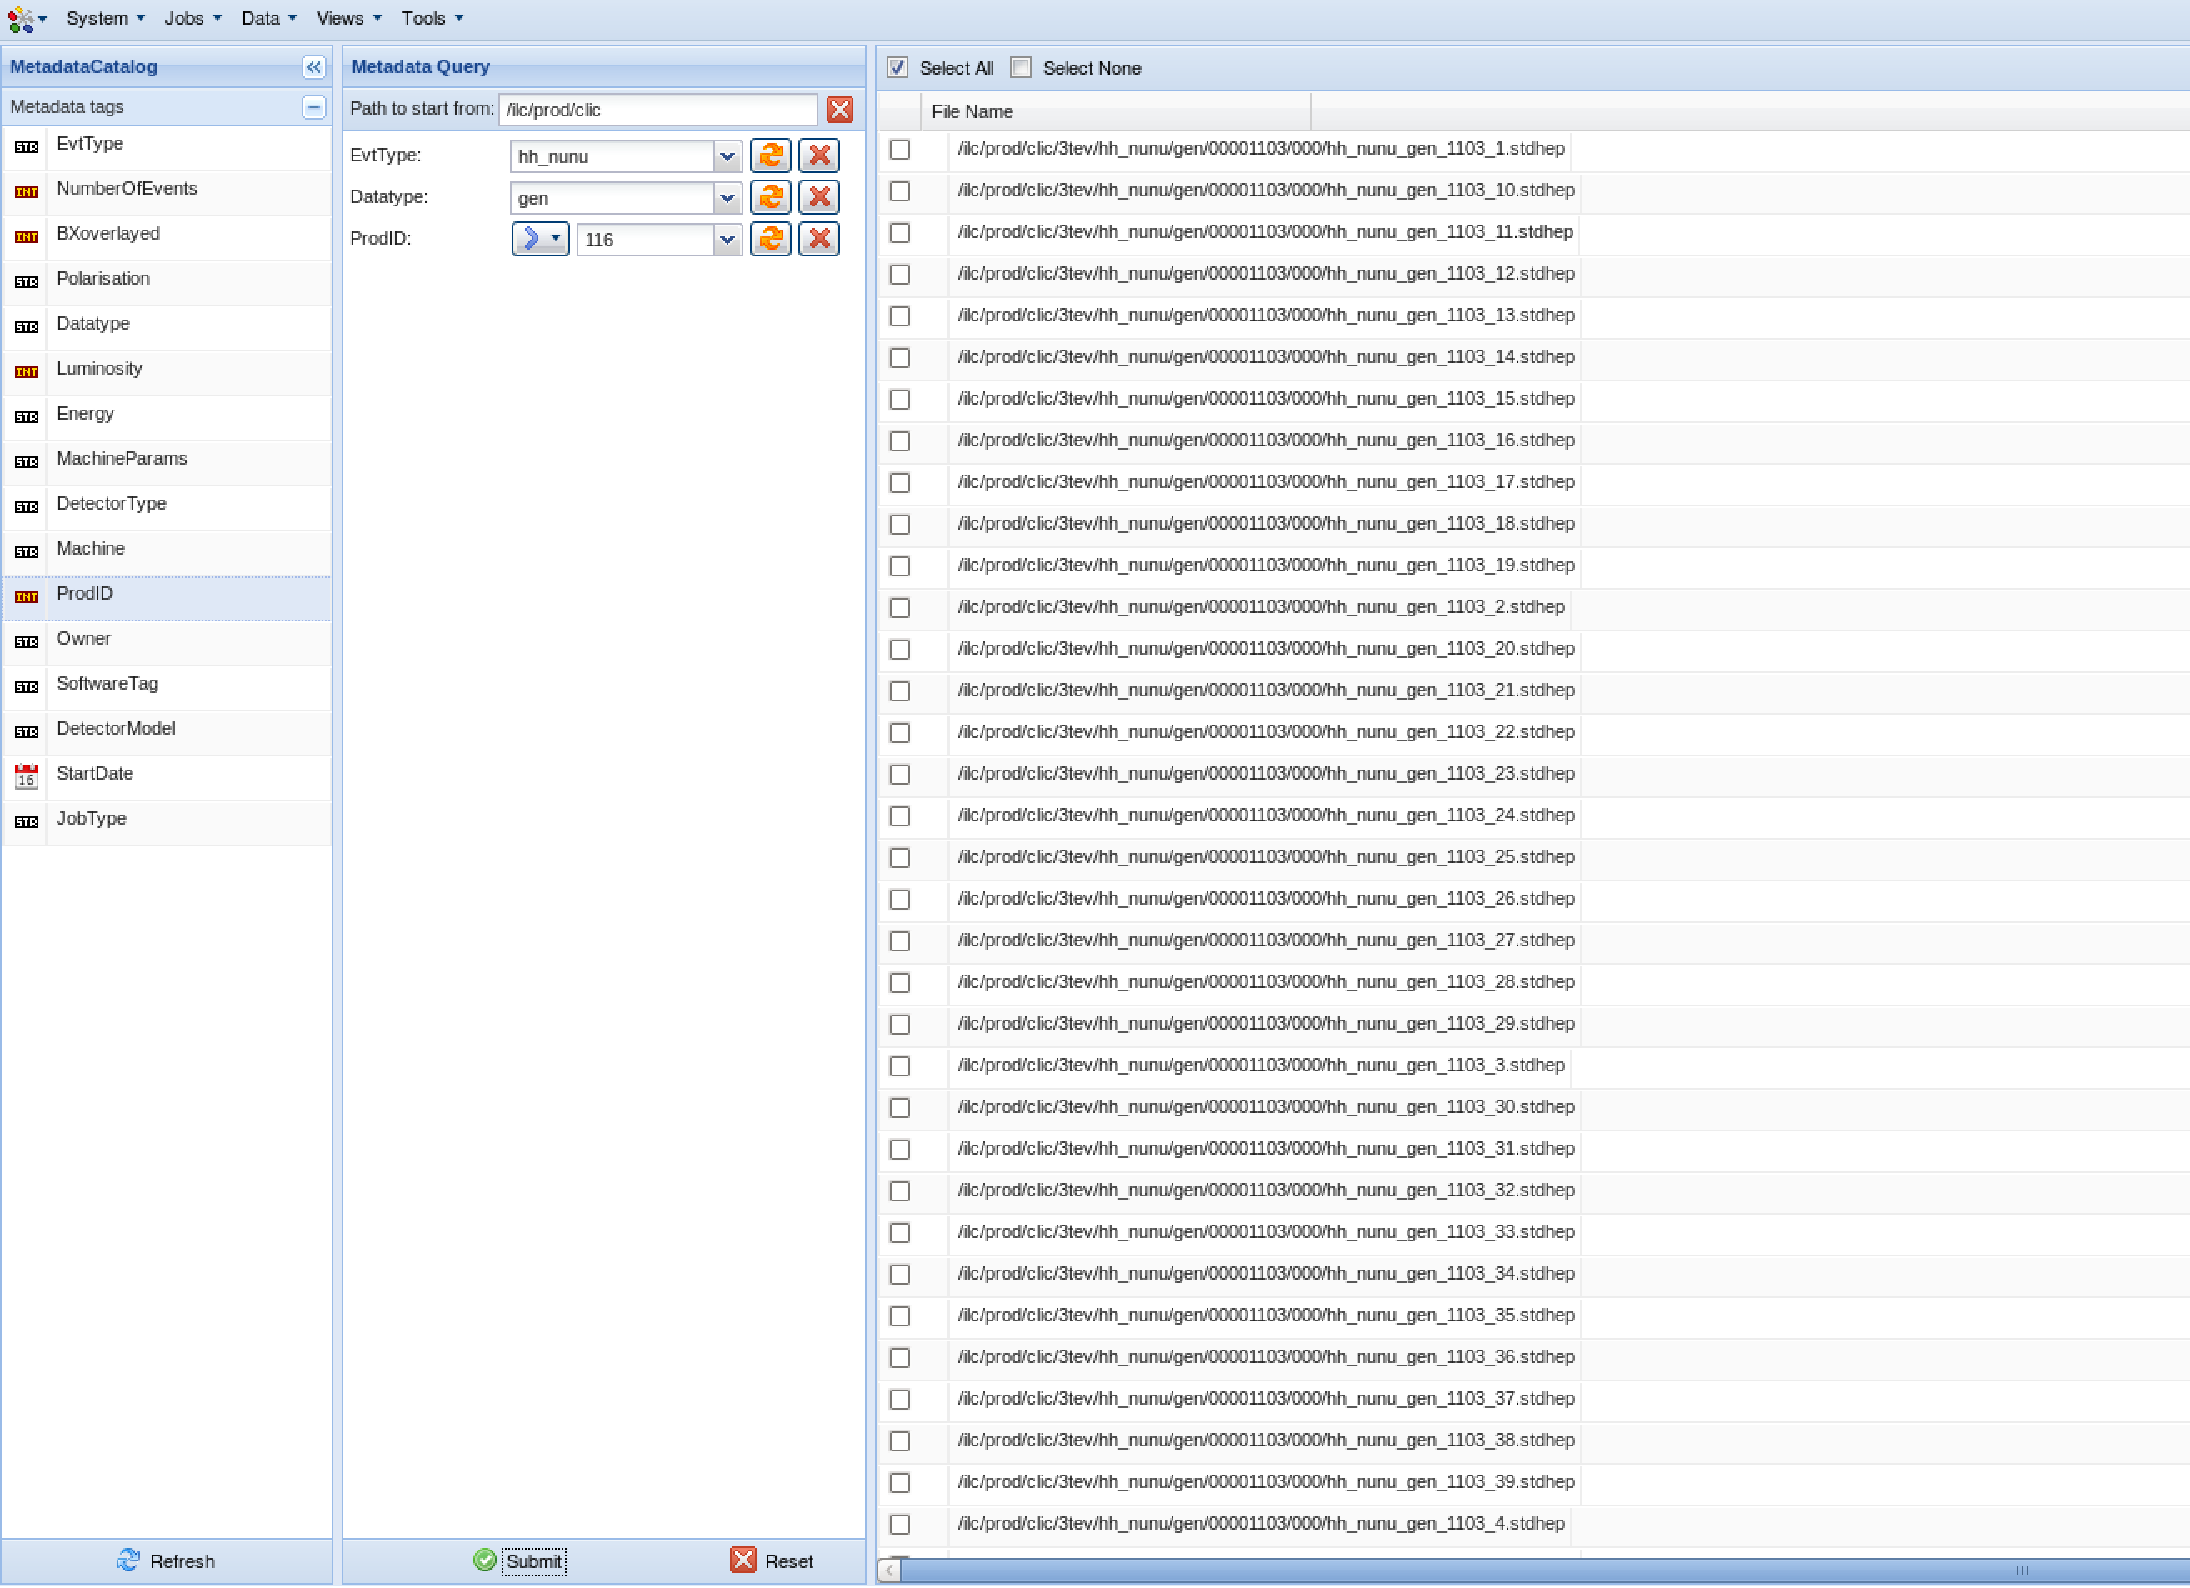
\includegraphics[width=.9\textwidth]{WebFC}~\\
\end{frame}

\subsection{Performance}
\label{sec:prefsfc}

\begin{frame}
  \frametitle{File catalog performance}
Timing for replica resolution:\\
~\\
\begin{columns}[c]
\column{6cm}
Many concurent clients:\\
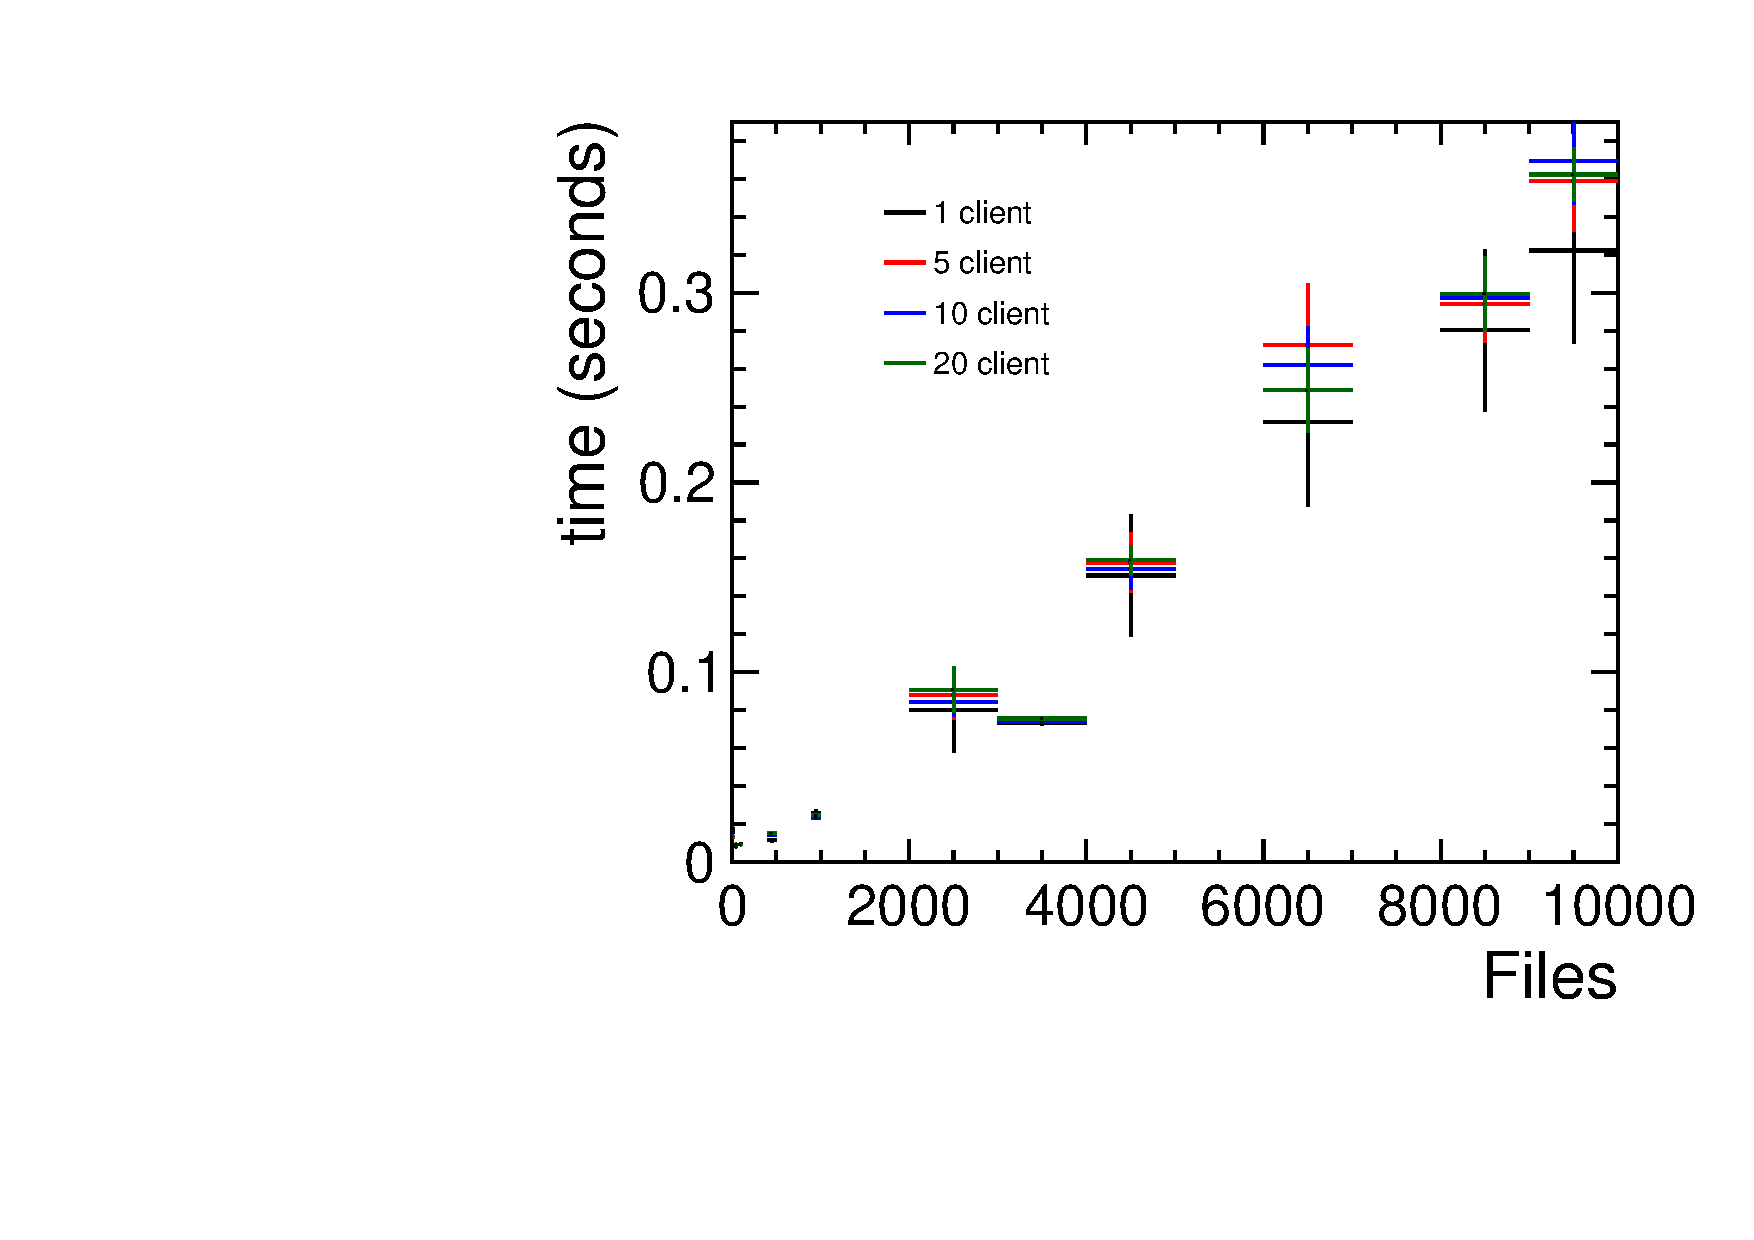
\includegraphics[width=\textwidth]{DFC_stats_lin_all}
\column{6cm}
One client:\\
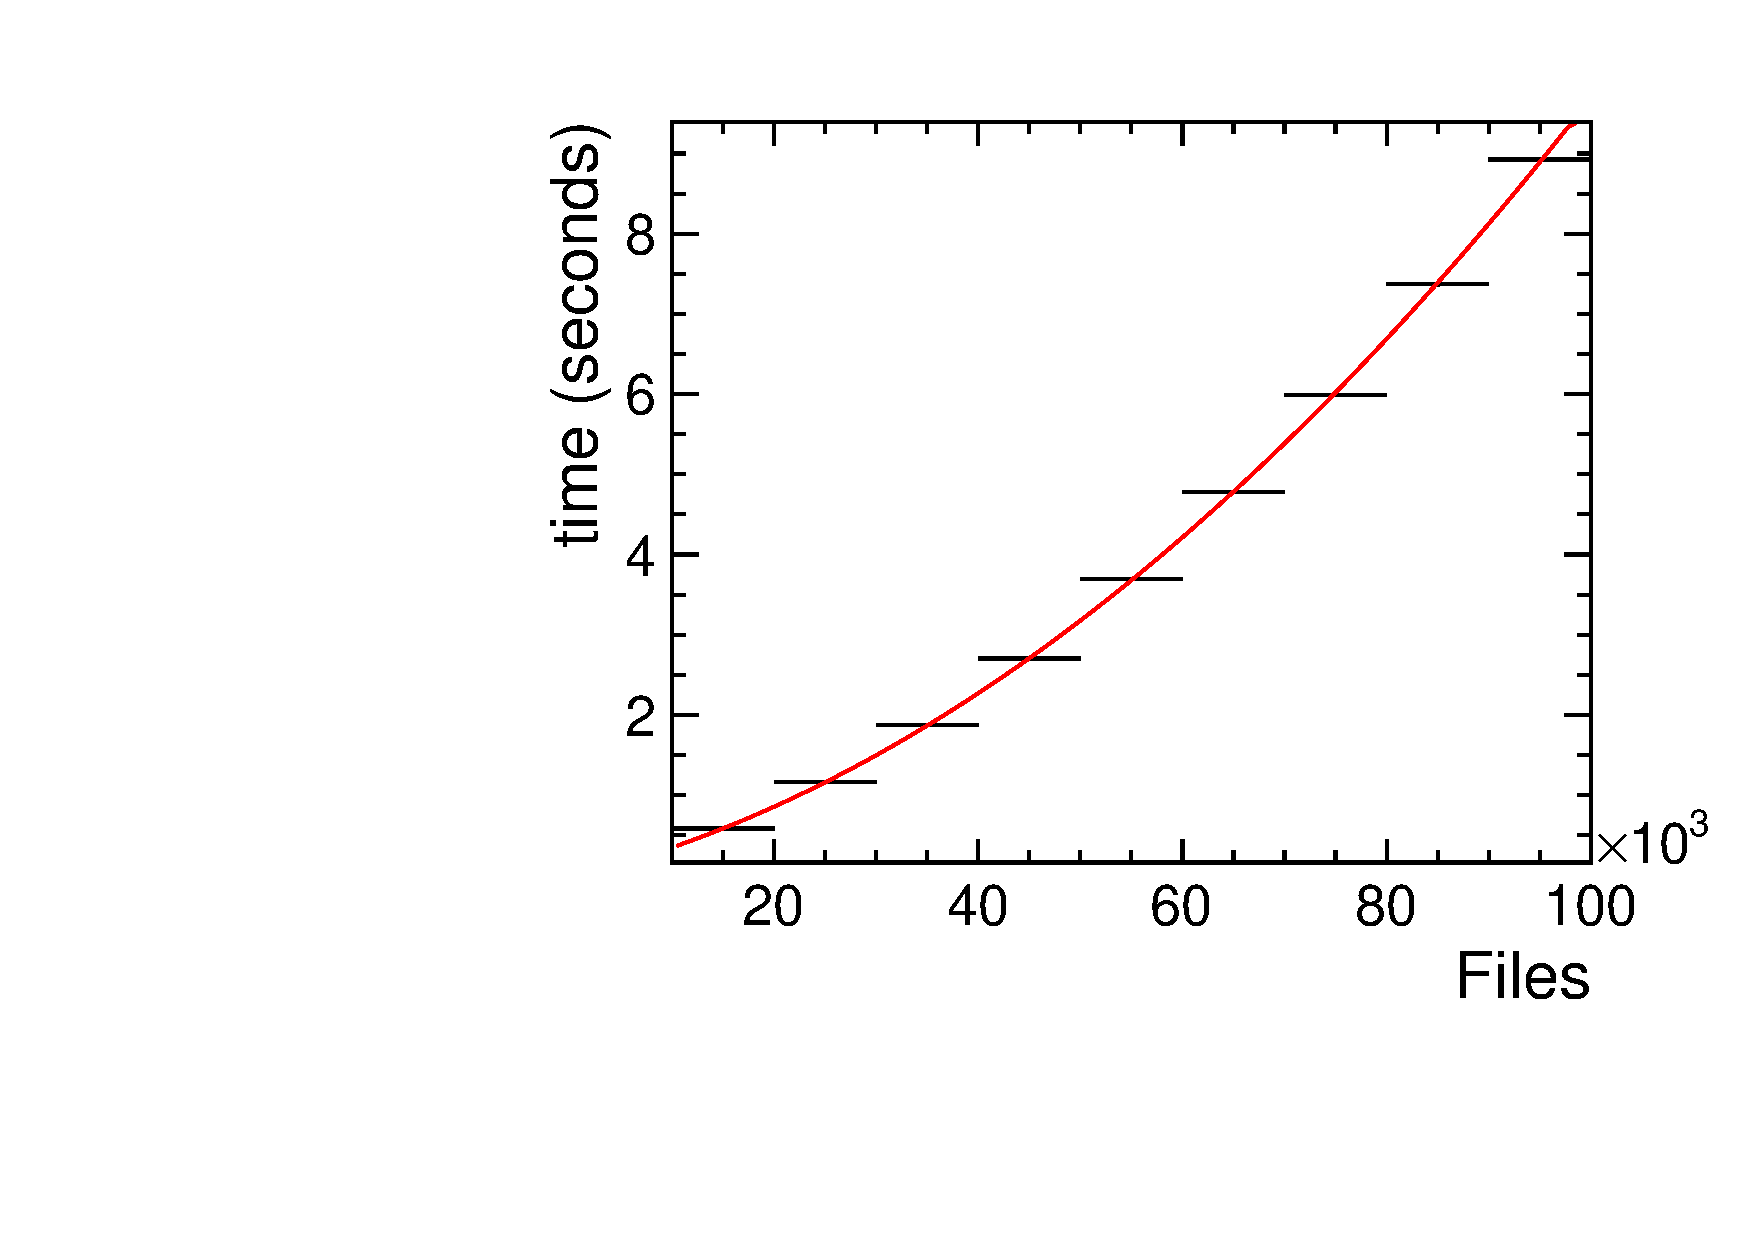
\includegraphics[width=\textwidth]{t_vs_f_nc1_zoom2_pol2}
\end{columns}
~\\
Meta data search times are compatible with those of the AMGA system
\end{frame}

\section{Production Management}
\label{sec:ts}

\begin{frame}
  \frametitle{Production system}
Idea: \alert{Apply a set of operations to a set of files automatically}
\begin{itemize}
\item {\color{NavyBlue}Generation} of a given channel at a given machine (with WHIZARD 1.95)
\item {\color{NavyBlue}Simulation, Reconstruction} of a given channel (ILD and SiD
  reconstruction chains)
\item {\color{NavyBlue}Transfer}: replication from one site to another
\item Additing new tasks at the Generation steps automatically implies
  the creation of Simulation/Reconstruction of the new files: \alert{data
  driven process}
\end{itemize}
~\\
All failing tasks that analyse files are reset: \alert{99.9\% of the data
produced was simulated/reconstructed} during the CLIC\_CDR production
\end{frame}

\section{ILCDIRAC Support}
\label{sec:support}

\begin{frame}
  \frametitle{Support to the users}
\begin{itemize}
 \item {\color{NavyBlue}Mailing lists}:
   \begin{itemize}
   \item for registering users: ilcdirac-register@cern.ch\\~\\
   \item for registered users: ilc-dirac@cern.ch\\~\\
   \end{itemize}
 \item {\color{NavyBlue}JIRA bug tracking}: https://its.cern.ch/jira/browse/ILCDIRAC
   \begin{itemize}
   \item CERN IT provides this service among others\\~\\
   \end{itemize}
 \item {\color{NavyBlue}Growing community} of users sharing tools\\~\\
 \item {\color{NavyBlue}Large support} from the DIRAC developers
\end{itemize}
\end{frame}

\section{Future plans}
\label{sec:future}

\begin{frame}
  \frametitle{Future plans}
  \begin{block}{Short term:}
  \begin{itemize}
  \item {\color{NavyBlue}Wiki} documentation: flexibility\\~\\
  \item {\color{NavyBlue}WHIZARD 2 and PHYSSIM} supported in ILCDIRAC:
    completeness
\end{itemize}
  \end{block}
~\\
\begin{block}{Longer term:}
\begin{itemize}
  \item {\color{NavyBlue}WHIZARD 2 process factory}: no precompiled
    binary needed, only \\process definition\\~\\
  \item {\color{NavyBlue}Configure} and {\color{NavyBlue}Run the applications locally}, no installation
    necessary, let DIRAC do it. {\color{ForestGreen}Ideal for testing.}
  \end{itemize}
\end{block}
\end{frame}

\section{Conclusion}
\label{sec:conc}
\begin{frame}
  \frametitle{Conclusion}
\begin{block}{ILCDIRAC is:}
\begin{itemize}
\item A \alert{fully functionnal grid solution} for the Linear Collider
  community
  \begin{itemize}
  \item Used for {\color{ForestGreen}CLIC CDR} and {\color{ForestGreen}ILC DBD} activities\\~\\
  \end{itemize}
\item Coming with an {\color{NavyBlue}intuitive/user friendly} interface\\
~\\
\item {\color{NavyBlue}Easily connected with any new resources} (Site, storage,
  etc.)\\
~\\
\item {\color{NavyBlue}Open source}\\
~\\
\item {\color{NavyBlue}Available} for any ILC VO member
\end{itemize}
\end{block}
\label{lastframe}
\end{frame}

\backupslides

\begin{frame}
  \frametitle{Site usage}
\centering
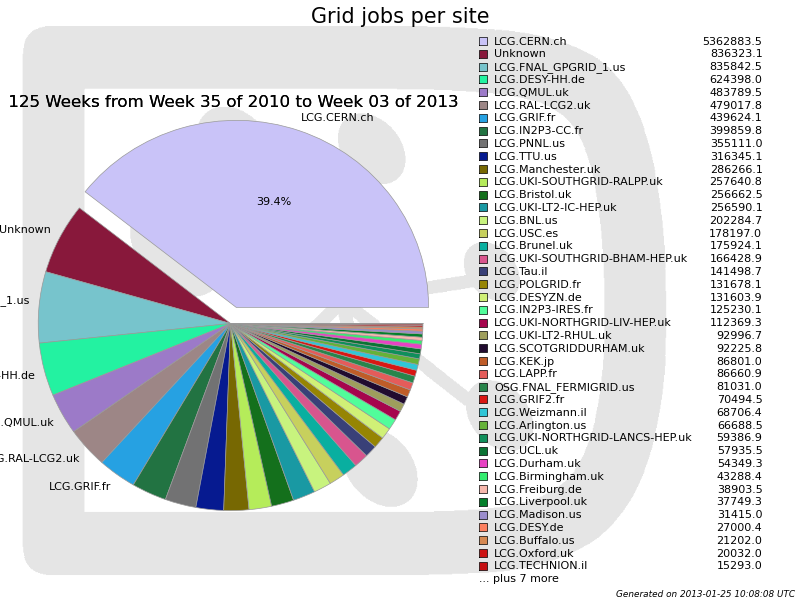
\includegraphics[width=0.9\textwidth]{PilotsPerSite}\\
\end{frame}
\end{document}


% Local Variables:
% TeX-PDF-mode: t
% End:
